\chapter{RTL 工程化接口、状态机与联调}
\label{ch:rtl-engineering}

\section{先确定正在编译的结构}
\code{rtl/rtl_sources.f} 是生产编译清单，实际列出22个\code{core}模块和2个\code{top}目录模块；另有2个include头文件，因此源码审计对象共26文件。完整数字顶层为\code{sar20_digital_core}；\code{sadc_enc}虽位于top目录，职责是温度计编码，并不是另一套ADC。\code{rtl/README.md}已改为当前入口，逐模块职责、内部观测点和完整接口时序另见\code{docs/rtl/RTL_ENGINEERING_GUIDE.md}。历史P1/P2记录保留自己的范围，不能用“13个模块”或“Flash始终在核外”的旧入口解释当前设计。

\begin{table}[H]\centering\small
\begin{tabularx}{\textwidth}{p{32mm}XX}
\toprule 精化选择&输入边界&实际控制与用途\\\midrule
\code{P_STRUCTURAL=1}，默认&7位Flash温度计、Flash有效、两路coarse及一路fine比较器valid/data&双9-bit seeded SAR、共享3-bit Flash、18-slice池；共享fine转换前代residue。\\
\code{P_STRUCTURAL=0}&外部9-bit粗码及ready、12-bit细码及ready&兼容原有码域oracle；phase8/14分别捕获完整粗细码。\\\bottomrule
\end{tabularx}
\caption{两种profile的实际含义。它们是精化参数而非运行时模式切换。结构模式内部使用\code{sadc_enc(P_B1=3)}，兼容模式保留完整码输入。}
\end{table}

两种结构共享物理系数、配置和精确定点重构，但前端握手不同。
结构模式的\code{cmp_valid}每次解决一个SAR位；兼容模式的\code{ready}只在完整码捕获截止沿有意义。
全部顺序逻辑使用统一\code{clk}上升沿和同步低有效复位。配置、比较器、ready/data均须满足该时钟的建立保持条件；RTL没有自动加入CDC。
\code{P_RECON_STAGES}是另一个精化参数，控制每拍展开的恢复除法位数，不能与上述两profile混同。

本轮工程整理展开压缩行、分开执行语句、统一缩进与运算符空格，明确模块的职责、接受沿、复位、取消、异常和综合观察点。
这次整理不通过重命名、重排表达式、增加流水或改变宏定义调整电路；有效SystemVerilog token和预处理指令必须逐项保持。
文本字节SHA改变时，先前Vivado证据仍只直接绑定其旧文件字节；交付清单另记录新文件身份与token比较，再辅以当前编译/回归。
这种比较证明表达式没有被改写，不能被称为形式等价工具签核。

\section{模块边界决定调试顺序}
\begingroup\small
\begin{longtable}{>{\raggedright\arraybackslash}p{39mm}>{\raggedright\arraybackslash}p{57mm}>{\raggedright\arraybackslash}p{47mm}}
\toprule 源码或模块&职责与保存的信息&先观察的信号\\\midrule\endfirsthead
\toprule 源码或模块&职责与保存的信息&先观察的信号\\\midrule\endhead
\code{analog_phase_ctrl}&计数与注册TP/AZ/参考/放大使能；不实现非重叠晶体管网络。&\code{phase/next_phase}及注册模拟使能。\\
\code{sar_trial_ctrl}&隔离pending trial与accepted code，保存忙状态与位序。&\code{busy/bit_index/trial_code/resolved_code/done}。\\
\code{sar_structural_ctrl}&双coarse、共享fine、deadline与bank交接的集成。&\code{bank/sid/coarse_ok/fine_ok/error_code}。\\
\code{slice_pool_ctrl}&前周期acquiring提升为converting，补集选下一组。&\code{primed/conversion_valid}、两组IDs与\code{cursor}。\\
\code{cal_sample_context}&冻结当前物理开关决策，下一周期交给fine。&\code{residue_valid/fine_valid/fine_id/fine_slices}。\\
\code{ctrl_fsm/slice_alloc}&兼容模式节拍与分配；不用结构模式截止表。&\code{ph/adv/sample_idx/seen_sample}。\\
\code{dem_state_gen/dem_addr_gen}&A/B状态推进和主/子阵列物理位置映射。&两组sid、捕获sid与逻辑位置。\\
\code{swap_decode/unit_therm}&粗码/dither/bridge到计数，再到物理开关与轨。&计数、\code{rdac_over}、开关掩码。\\
\code{dither_gen/rdac_drv}&生成离散随机码；后者只注册数字命令。&\code{valid/load}及输出开关。\\
\code{weight_store}&权重、写满位图、共享旧系数选择和精确行和。&\code{accept/written/row_q/old_by_slice}。\\
\code{calib_regs}&三标量、四控制位与配置validate。&\code{scalar_written/cfg_ready/err_code}。\\
\code{cal_weight_reduce}&物理集合及掩码归约得到\(T,G,R\)。&\code{sum_W/sum_Wa/rails/invalid_slice}。\\
\code{adc2_dec/cal_residue_mac}&bin center及half-even；快照后的受检MAC。&\code{fine_q/a1/any_ovf}。\\
\code{div_floor}&幅度恢复除法、宽分母、负数floor修正。&\code{run/cnt/rem/quo/q/done/err}。\\
\code{recon_core}&接受、快照、MAC launch、除法及完成事件。&\code{stage_b/div_busy/div_done/sample_id_r}。\\
\code{cal_output_stage/status_regs}&事务code/ID/flags原子提交；组合错误码透传和粘滞事件。&\code{complete/dout_valid/result_flags/status_word}。\\
\code{sadc_enc}&平衡计数树；不包含比较器阵列。&\code{cmp_raw/count_tree/sadc_code}。\\
\code{sar20_digital_core}&总线仲裁、精化profile及数字核集成。&\code{cfg_bus_ok/ctrl_seq/launch_recon/dout_sample_id}。\\\bottomrule
\end{longtable}
\endgroup

这些都是现有内部网或端口，可供testbench波形定位；本次没有引入宽调试总线或FIFO。
调试时先分清控制是否接受本笔事务，再检查已捕获数据，最后定位算术。
例如没有\code{launch_recon}时，应先查valid/deadline/priming；不能先怀疑MAC公式。
\code{rtl_params.vh}由参数导出器生成，改变数值规格须更新来源配置和漂移检查；\code{rtl_error_codes.vh}是静态接口常量。

\section{前沿、相位区间与非阻塞赋值}
本章所有“phase \(p\)沿”都指上升沿到来前\code{phase=p}。
同沿\code{phase<=next_phase}与注册模拟使能一起更新，更新后的电平占据下一相位区间。
因此必须区分三个时点：沿前接受条件、沿上采样的旧数据、NBA完成后的新寄存器电平。

以默认coarse截止为例：phase7沿是第六次粗比较的最晚有效沿，该沿还把\code{coarse_cancel}置1；进入phase8区间后，\code{coarse_done=1}与cancel同时存在。
phase8沿控制器读取旧done并锁存\code{coarse_ok}，SAR读取旧cancel清busy/done；随后进入phase9。
把phase8区间的done误写成“phase8沿又作了一次比较”，会多给一拍预算并遗漏取消语义。

同一上升沿的多个\code{always_ff}均读取旧值，给本设计带来四项刻意的因果关系。
第一，\code{sid<=sid_a/sid_b}与DEM推进同沿，当前样本用旧sid；推进后的sid留给下一次该bank。
第二，pool把旧acquiring提升为converting，新的acquiring由旧cursor扫描；同沿PRNG改变的是下次origin。
第三，SAR的resolved更新与valid脉冲在一个沿产生，RDAC下一沿消费已决码，从未把未确认trial送入重构开关状态。
第四，重构完成沿可同时接受下一start，提交读取旧\code{sample_id_r}，新ID于NBA后成为下一笔快照。

在波形和文本trace里应同时保存edge编号、沿前phase和NBA后值。
只根据日志里打印的phase判断“哪一沿接受”会产生一拍偏差；图中边上的条件则必须来自沿前条件。
解释状态机是阅读代码的工具，实际有效性还由后述自检trace、独立参考和原始日志判断。

\section{结构模式的16相位与启动填充}
默认\code{P_RESIDUE_CAPTURE=9/P_REF_ON=10}形成表\ref{tab:eng-structural-phase}。
表中current与previous指事务前后关系；它们不是保证从0或1开始的输出ID编号。
相位保持固定16拍，不等待比较器valid；缺少任何必须判决时在deadline取消未完成转换并记录错误。

\begin{table}[H]\centering\small
\begin{tabularx}{\textwidth}{p{21mm}Xp{34mm}}
\toprule 沿前phase&本沿数字事务&样本归属\\\midrule
0&交换coarse bank；旧residue转fine；捕获dither/injection，清两ok位。&fine来自前代，coarse准备当前代。\\
1&pool晋升；Flash seed启动coarse；valid context启动fine；保存旧sid/random输出。&两代并行。\\
2--7&六次最早可用的coarse比较，完成未由Flash决定的6位。&当前粗码。\\
2--8&RDAC接收上个沿resolved update；2沿可写seed，8沿可写最终码。&当前已决开关。\\
8&接收coarse done；SAR取消清busy/done。&决定当前residue有效性。\\
9&捕获当前物理IDs、掩码、轨、模式、注入与有效性。&保存供下一周期fine。\\
2--13&十二次最早可用的fine比较。&前代residue。\\
14&接收fine done/code；fine取消清忙。&前代细码。\\
15&context有效、fine成功且recon空闲时启动重构。&冻结context的ID。\\\bottomrule
\end{tabularx}
\caption{默认结构模式前沿事务。2--8行是RDAC更新窗口，与粗比较窗口重叠，不是增加的相位。}
\label{tab:eng-structural-phase}
\end{table}

\begin{figure}[H]\centering
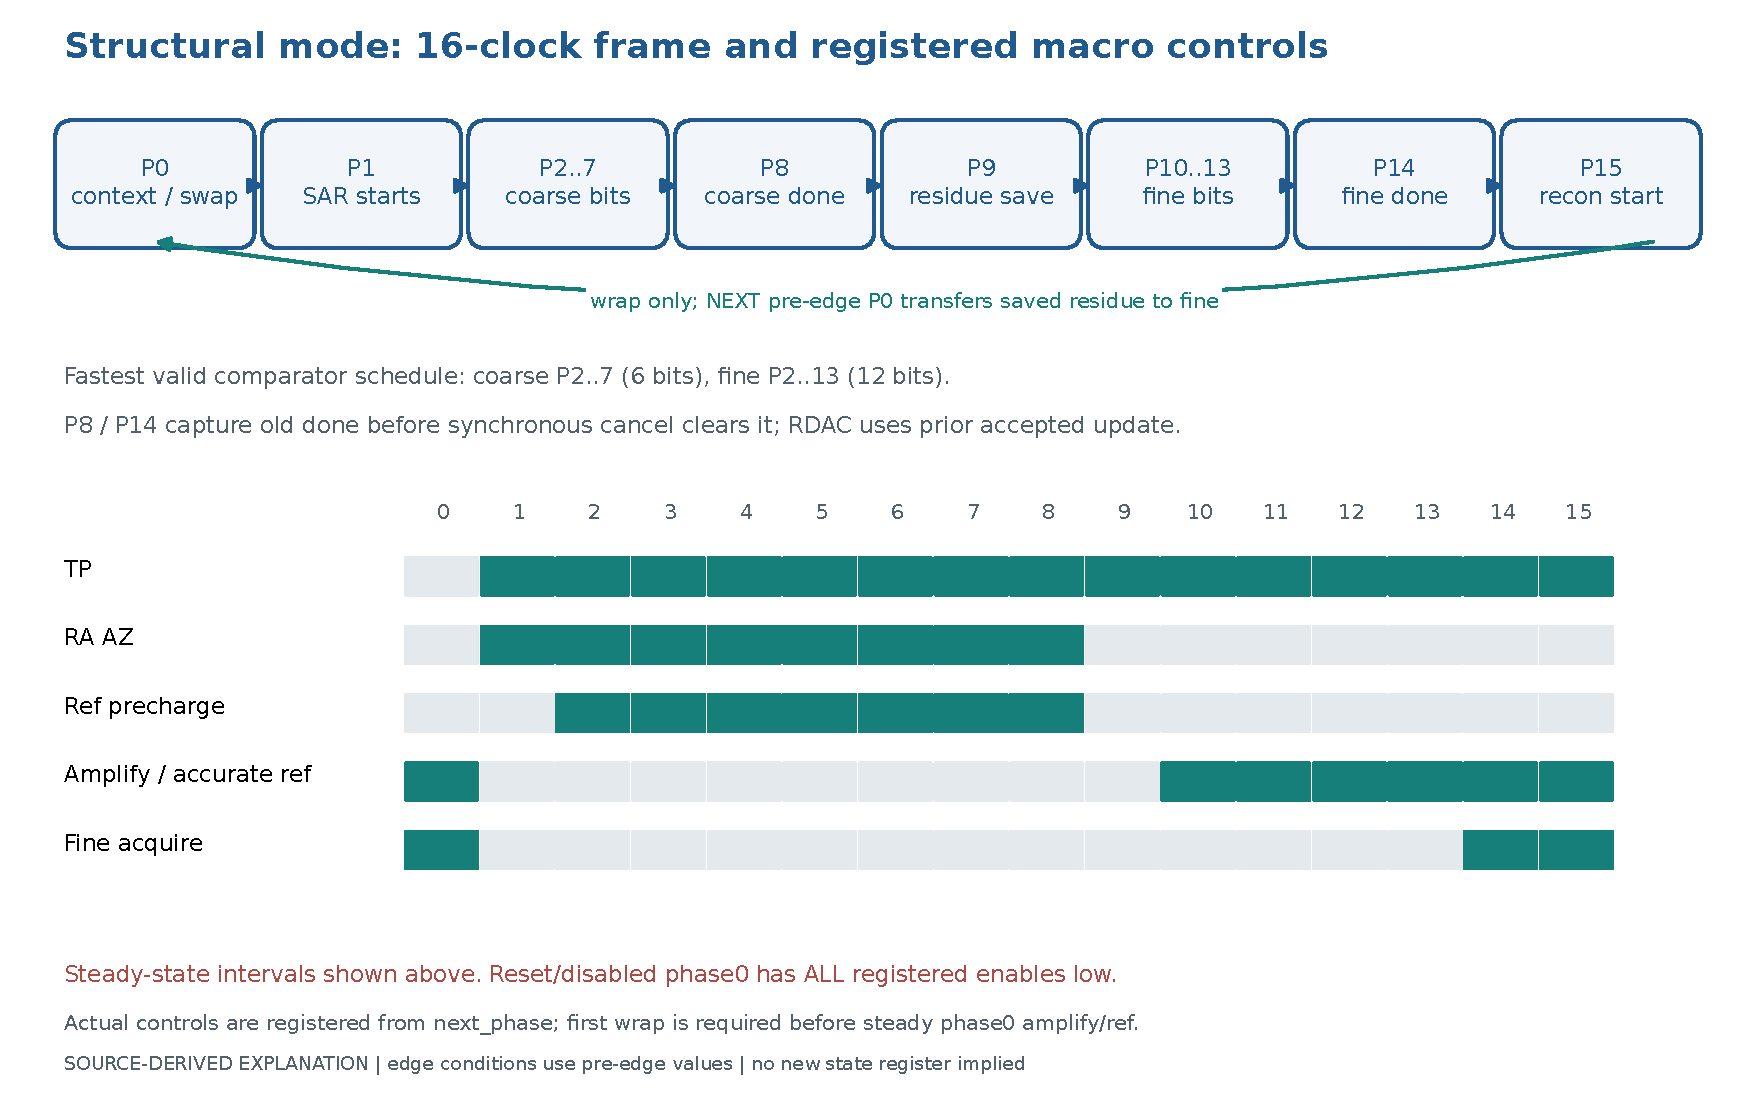
\includegraphics[width=0.96\textwidth]{figures/44_structural_phase_fsm.pdf}
\caption{按当前控制源码绘制的结构相位与重叠事务解释图。图不是仿真证明，也不是原芯片晶体管连接或其异步SAR时序披露。沿前phase与沿后注册输出必须分别阅读。}
\label{fig:eng-structural-phase}
\end{figure}

注册模拟电平采用look-ahead解码。稳态TP为phase1--15；AZ为1--8，precharge为2--8；amplify和accurate reference为0及10--15。
flash acquisition仅phase1低，fine acquisition在0/14/15高；coarse cancel占8/9，fine cancel占14/15。
默认phase9两种参考使能都关闭，但这只是数字死区，不能替代真实模拟非重叠、开关延迟和参考建立验证。
\code{compare_enable}是电平使能，不能画成比较器复位时钟。

启动阶段有两层填充。
复位后phase=0而全部注册模拟输出为0；稳态phase0的amplify/reference高电平只有首次wrap后才出现。
pool初始acquiring为IDs0--7，converting无效；第一次advance把primed置1，但\code{conversion_valid}读到旧primed=0，第二次才有效。
当前有效residue还要在下周期phase0转fine，随后fine完成才可重构。
因此首轮没有输出不等于RTL失败，判断应依据primed、\code{conversion_valid/residue_valid/fine_valid}的链，而不能删掉priming以让图更早显示成功。

\section{SAR状态不是试探码等于已决码}
\code{sar_trial_ctrl}以busy编码实际状态，没有额外枚举寄存器。
\code{start}在idle时只留下seed高位，并把首个未决位设成trial；resolved\_valid随seed初始化置1，给RDAC一次已决高位更新。
比较器约定为\code{cmp_ge=1}接受当前DAC试探位。busy且cmp\_valid时，接受/拒绝该位，再试探下一位；cmp\_valid=0保持位序和trial，不重复消耗该位。
最后bit\_index=0的有效判决使busy清零、done和resolved\_valid各高一拍。

\begin{figure}[H]\centering
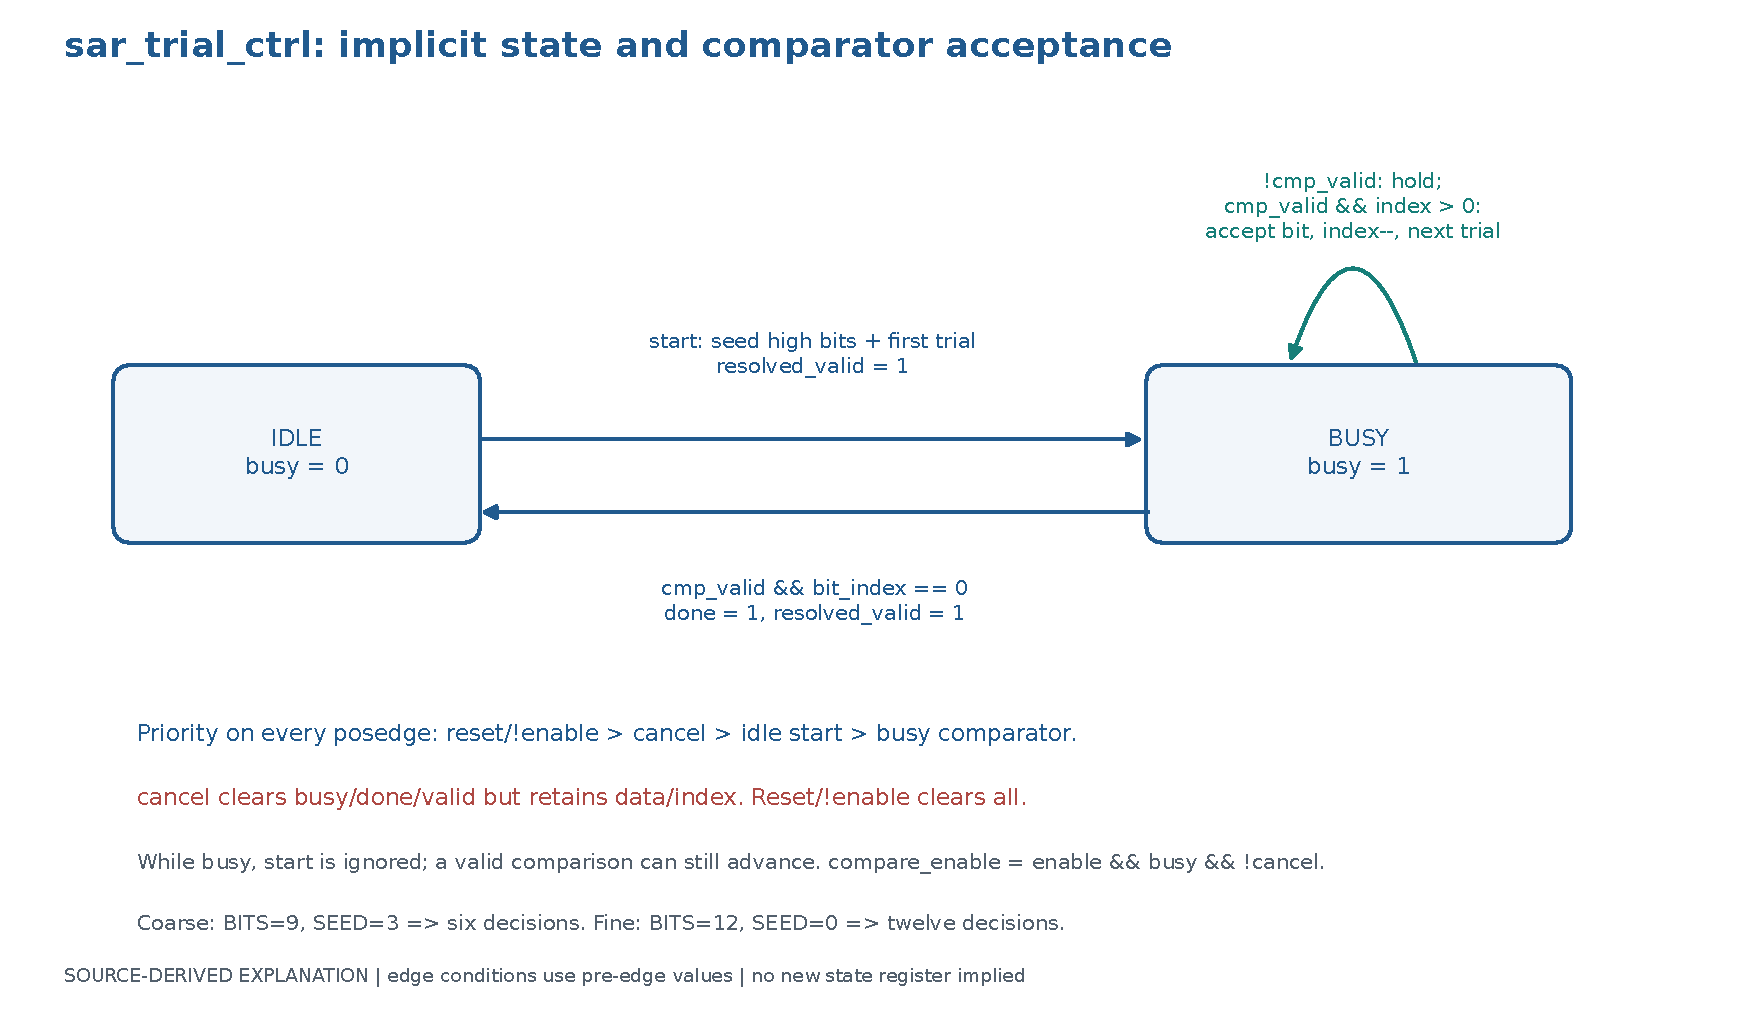
\includegraphics[width=0.94\textwidth]{figures/45_sar_trial_fsm.pdf}
\caption{SAR控制的IDLE/BUSY逻辑状态解释图，反映当前busy/index编码与转移优先级。它不是仿真证明；转移需由有效比较、停顿、busy start、cancel与reset用例实际覆盖。}
\label{fig:eng-sar}
\end{figure}

前沿优先级严格为reset/disable、cancel、idle start、busy valid comparison。
cancel清忙与事件，但保留trial/resolved/index；disable和reset清全部状态。
busy时start被忽略，但同沿cmp\_valid仍推进；idle start与cmp\_valid同沿只执行start。
\code{compare_enable=enable \&\& busy \&\& !cancel}没有异步rst\_n门控，reset关系必须按同步沿绘制。
粗SAR默认从3位seed解决余下6位，fine没有seed须作12次；不能把两者画成相同决策次数。

控制与电路的关系到此止步：seeded binary及同步valid是本工程实现选择。
图不能证明原论文使用同一比较器复位网络、SAR延迟或bit radix。
coarse\_trial/fine\_trial输出是宏接口命令，采样电容、比较器和DAC实际拓扑仍需模拟原理图与瞬态结果。

\section{前代fine上下文防止跨样本污染}
\code{cal_sample_context}有residue与fine两组信息，不把所有状态放在一个“当前样本”寄存器里。
phase9将当前ID、8个物理slice ID、主/子开关掩码、dither轨、sampling flag和injection保存；下一周期phase0把保存值搬入fine端口。
fine量化上一residue时，coarse bank、pool、DEM和当前输入已进入下一代，但fine重构仍读冻结packet。
系数在整个配置epoch内保持不变，因而物理地址和权重的对应不被新配置打断。

当前residue有效条件为\code{conv_valid \&\& coarse_ok}；RDAC范围错误单独冻结为\code{residue_bad}。
\code{fine_analog_bad}在quiet transfer时取当时analog\_bad或旧residue\_bad；不能把其全部解释为phase9采样。
顶层模拟异常通过状态通道报告，与输出算术flags并非同一字段。
这些边界应在波形中单列，避免细码到轨就被误判成模拟过载。

两个strobe在默认相位中分离。
若测试人为同沿assert residue\_capture与quiet\_sample，NBA使fine收到旧residue，后写residue\_valid=0优先；没有同沿新residue旁路。
所以任意“pipeline优化”都须保存同样的ID、物理决策、模式、注入、valid和异常归属，不可直接换成live DEM或当期粗码。

兼容模式另外处理：phase8捕获完整粗码，phase14同时捕获细码、注入和模拟异常，15才条件启动。
ready是截止有效性，不是等待请求；\code{ctrl_fsm}的sample0、DEM10、RDAC11与结构模式的phase1推进不同。
停机或未配置时组合脉冲由adv立即屏蔽，下一沿phase归0；sample\_idx仅reset清零，停机时保持。
顶层配置后连续运行，兼容核的内部run不是新增外部启动接口。

\section{重构状态、精确延迟与输出资格}
重构接受条件为\code{cfg_ready \&\& start \&\& !busy}。
同沿快照已归约的\(T,G,R\)、后端bin center、offset、injection、ID和后端异常；下一沿才求本样本MAC并保存其异常。
若在接受沿就锁存组合MAC异常，将读到前笔快照，错误会错配一笔。
\code{stage_b}对应MAC\_LAUNCH，除法器run对应DIV\_RUN，div\_done对应待提交事件。

\begin{figure}[H]\centering
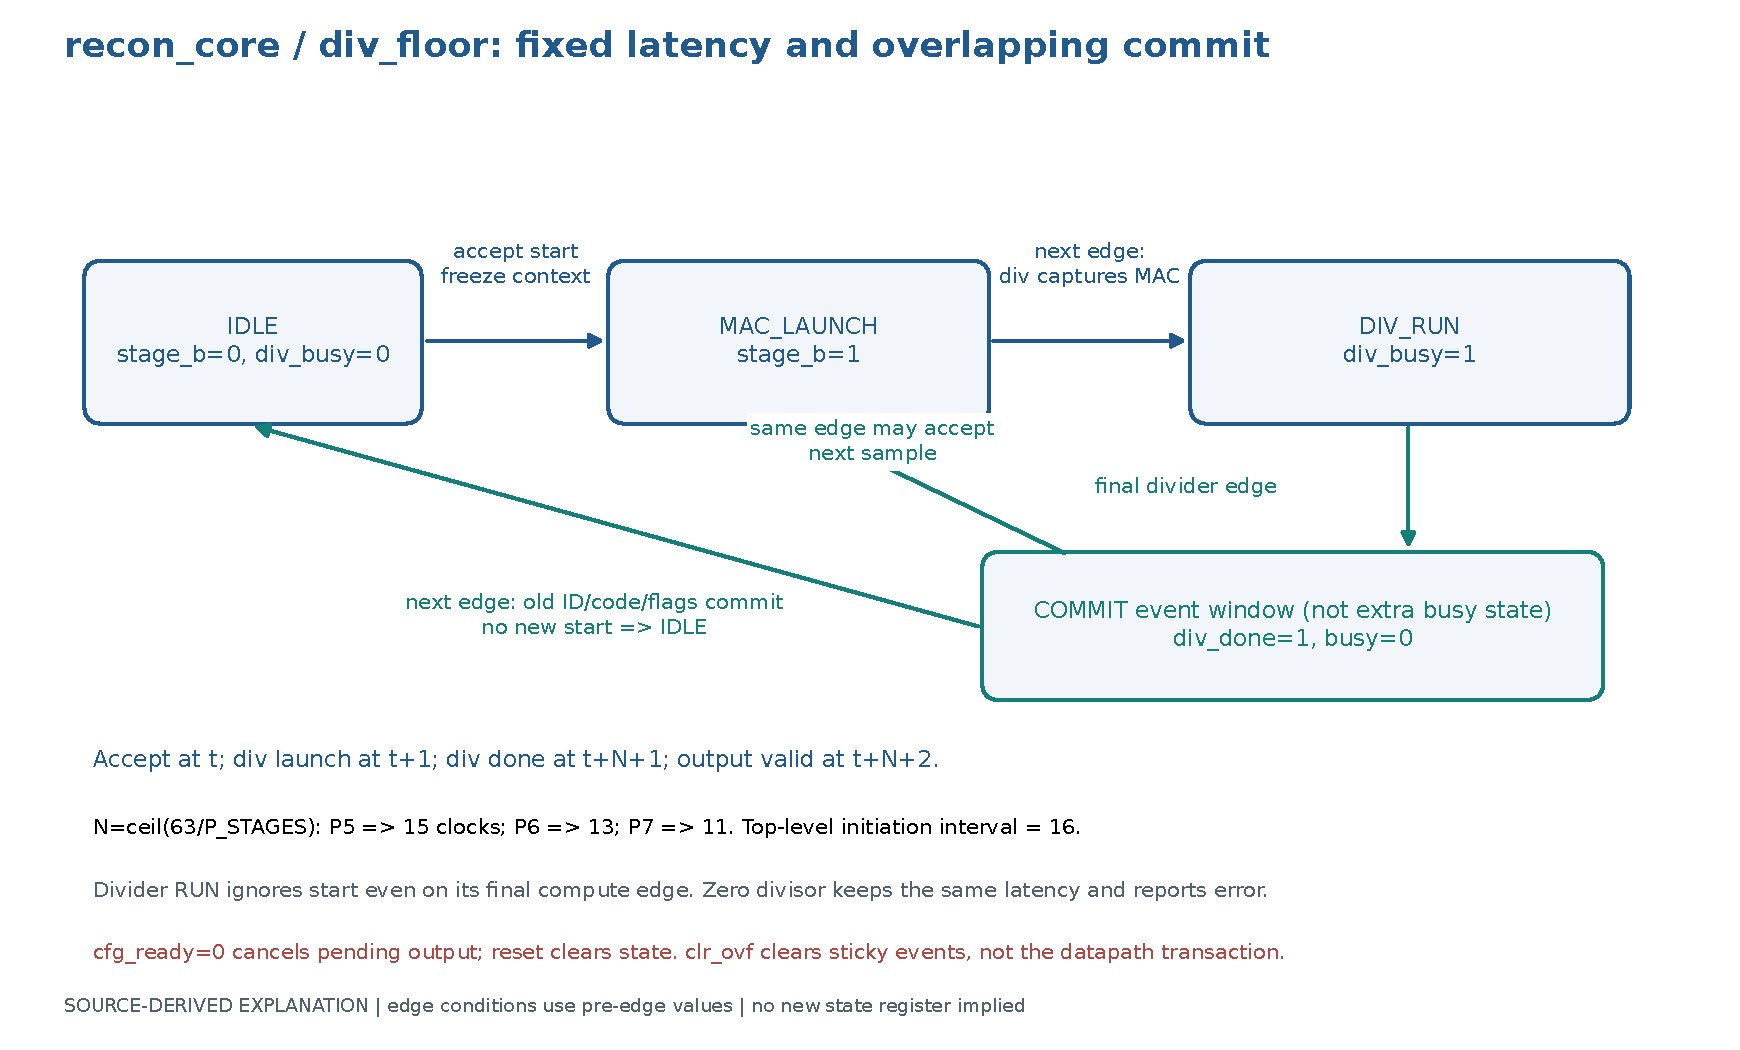
\includegraphics[width=0.94\textwidth]{figures/46_reconstruction_fsm.pdf}
\caption{由stage\_b、div\_busy和div\_done解释的重构流程图。COMMIT是事件窗口，没有独立state寄存器且此时busy已低；图不是仿真证明，不能据图增加一拍或声称形式等价。}
\label{fig:eng-recon}
\end{figure}

恢复除法每拍处理\code{P_RECON_STAGES}个商位，总迭代数为
\begin{equation}
N_{\rm cyc}=\left\lceil\frac{63}{P_{\rm RECON\_STAGES}}\right\rceil,
\qquad L_{\rm start\rightarrow valid}=N_{\rm cyc}+2.
\end{equation}
P5/P6/P7分别是15/13/11个完整时钟间隔，不是纳秒，也不是把起点和终点同时计入的沿数。
顶层允许阶段数5--63以守住16拍帧预算；每拍展开更多位会加深组合路径，改参数后须重验帧启动、ID、flags和STA。
除法done产生时busy已低，下个提交沿可接受下一start；输出读取旧ID与旧商，不增加额外busy拍。

\code{dout_flags[4:0]}为\{clip\_high,clip\_low,adc2\_ovf,gain\_err,acc\_ovf\}。
acc\_ovf或gain\_err仍产生dout\_valid和本次ID/flags，但保留最后合法字及clip状态；单独adc2\_ovf不阻止码更新。
所以valid是完成事件，不是无条件正确码的证书。\code{clr_ovf}只清粘滞事件，同沿新错误优先再置位；配置取消另由cfg\_ready/epoch reset中止流水并清输出。
这些异常条件不能为了更短延迟或更小面积而删除。

\section{配置状态与完整重载}
配置图解释现有cfg\_ready、ctrl\_seq、written与scalar\_written，并非新增状态枚举。
总线没有独立ready/ack，正常\code{rst_n=1}的上升沿，写入是否接受由\code{cfg_bus_ok}确定；reset沿即使组合条件为高仍优先复位；回读为组合数据。
全部写要求未生效、未validate、未clear、ctrl\_seq=0，并满足地址/位宽/数值守卫。
窗口地址\code{0x2000+s*0x100}先选择物理slice，再以\code{0x0000+8*u}写71项权重；窗口与权重不能同沿旁路。
\code{0x1000/1008/1010}依次为offset/min/max，\code{0x1018}为四控制位，\code{0x1020}仅状态只读。

\begin{figure}[H]\centering
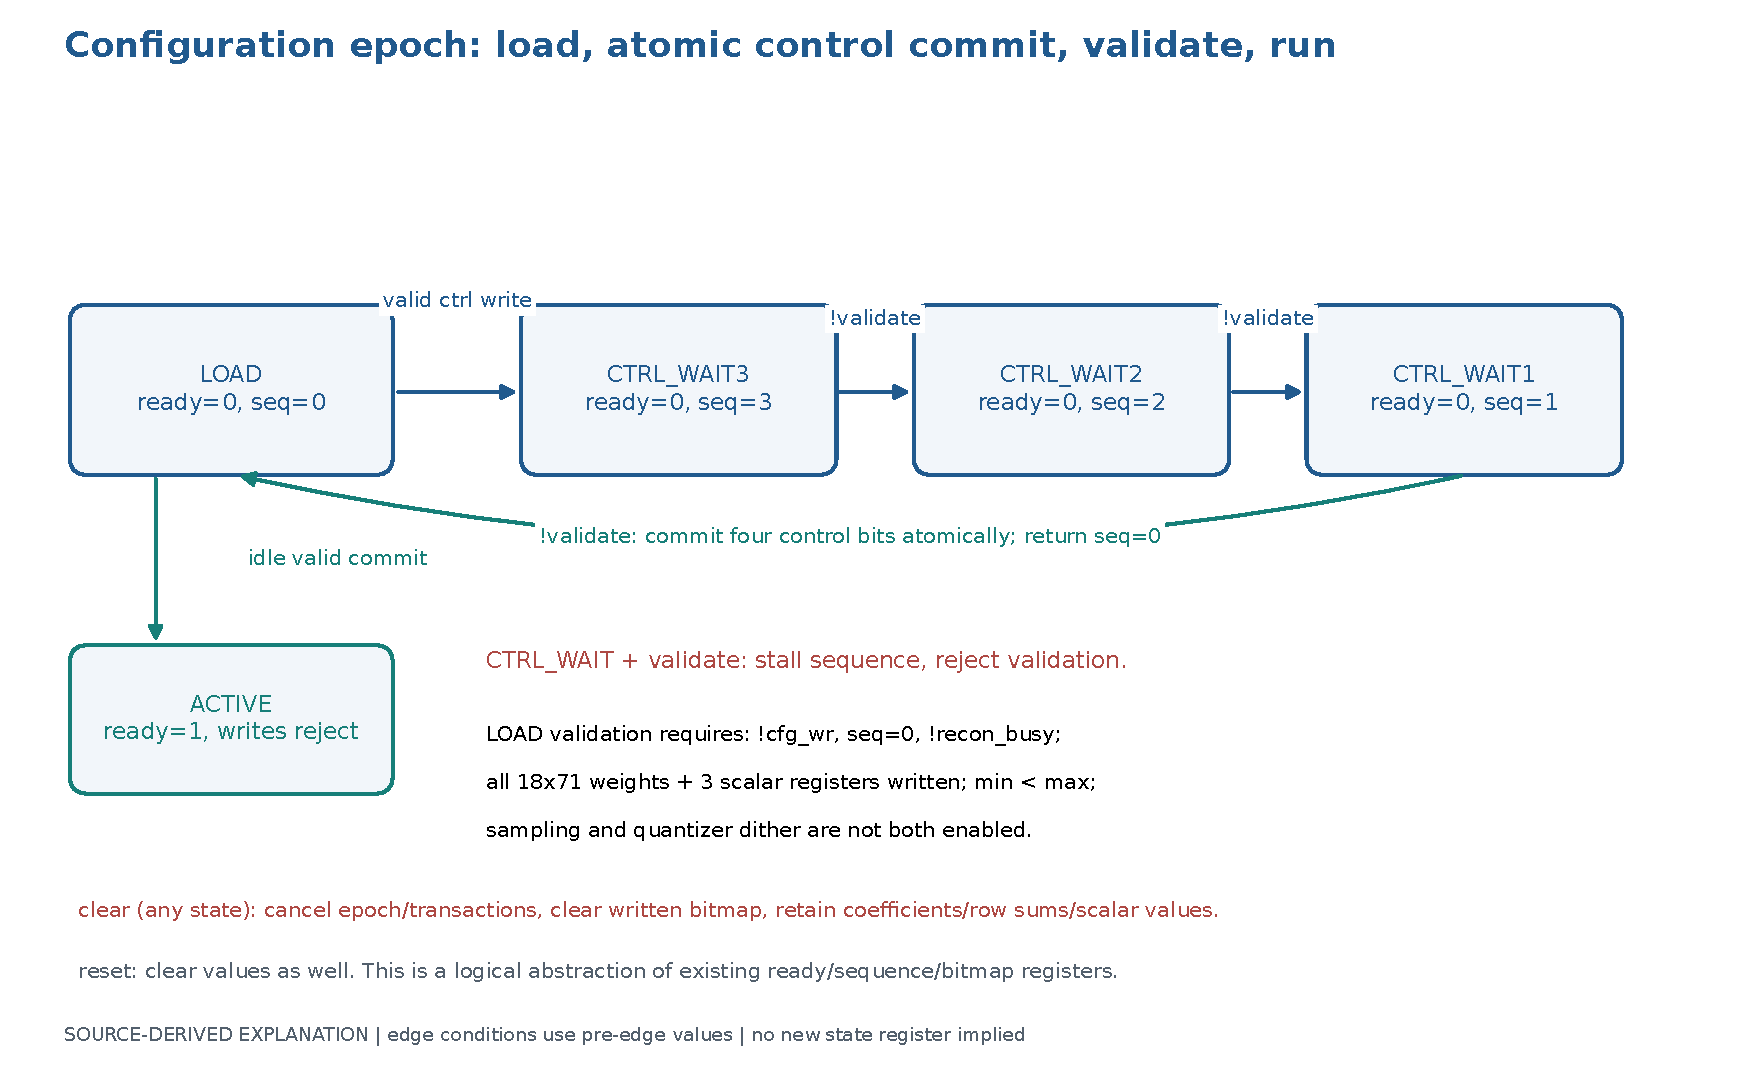
\includegraphics[width=0.95\textwidth]{figures/47_configuration_fsm.pdf}
\caption{配置LOAD、控制等待与ACTIVE的逻辑状态解释图。clear和reset效果不同，validate冲突保持等待序列；图不是仿真证明，实际拒写/提交/取消须由配置测试观察。}
\label{fig:eng-config}
\end{figure}

接受四控制位写的沿捕获bits并令ctrl\_seq=3；后三沿依次3→2→1→0，仅旧seq=1的第三沿原子安装四位。
等待中拒绝其他写；validate冲突暂停seq并拒绝提交，不能使pending control提前生效。
正确提交须raw cfg\_wr=0、ctrl\_seq=0、recon不忙、1278权重与三标量在本epoch都写齐、min<max，并且sampling/quantizer不同时开启。
提交冲突保留原ready；合法性失败报告具体错误。ACTIVE中系数与控制锁定，不支持无停机改写。

clear最高优先，撤销ready、清written/scalar完成位和pending control、复位窗口并取消数字事务；权重、精确行和及标量数值保留供读回。
旧读回非零不代表新epoch已完整，新epoch仍要逐项重载。
写权重替换的行和必须为\(H'=H-W_{old}+W_{new}\)，不能在bitmap清零后把旧数值当零。
rst\_n复位才清数值。顶层错误读回依次优先总线、配置、权重拒绝、profile控制；最新错误与粘滞状态应分开观察。

\section{把解释图与真实trace一起审阅}
解释图有助于定位转移，但有效性还需实际接受事件、状态和输出的关联。
本工程入口\code{tools/run_open_rtl.py}当前注册23bench（原22项及新增工程FSM见证）及结构、兼容、独立编码器3种严格lint；缺工具、编译失败或无完成标记均失败。
协议定位优先看SAR、structure、config和recon定向bench，再检查完整顶层；各自检查数单位不同，不相加冒充同一覆盖率。

\begin{table}[H]\centering\small
\begin{tabularx}{\textwidth}{p{34mm}XX}
\toprule 问题&先查的接受/状态&随后数据归属\\\midrule
\code{cfg_ready}不生效&完整位图、三标量位、ctrl\_seq、提交冲突&min/max、模式位、实际\code{cfg_bus_ok}。\\
启动不出码&primed、conv/context valid、done截止&前代packet ID、phase15 launch。\\
粗码偏一位&trial/resolved/index与valid&RDAC消费更新是否晚一沿。\\
输出错配样本&residue/fine/\code{sample_id_r}&提交沿与新start同沿的旧ID。\\
clear后旧输出&epoch reset、\code{cfg_ready}、div状态&valid被取消、完整位图重新建立。\\
码异常而日志全绿&每笔flags与status&\(T,G,R,F,O,I\)快照对独立整数oracle。\\\bottomrule
\end{tabularx}
\caption{从控制接受条件到数据快照的定位顺序；内部观测不新增生产调试端口。}
\end{table}

\begin{figure}[H]\centering
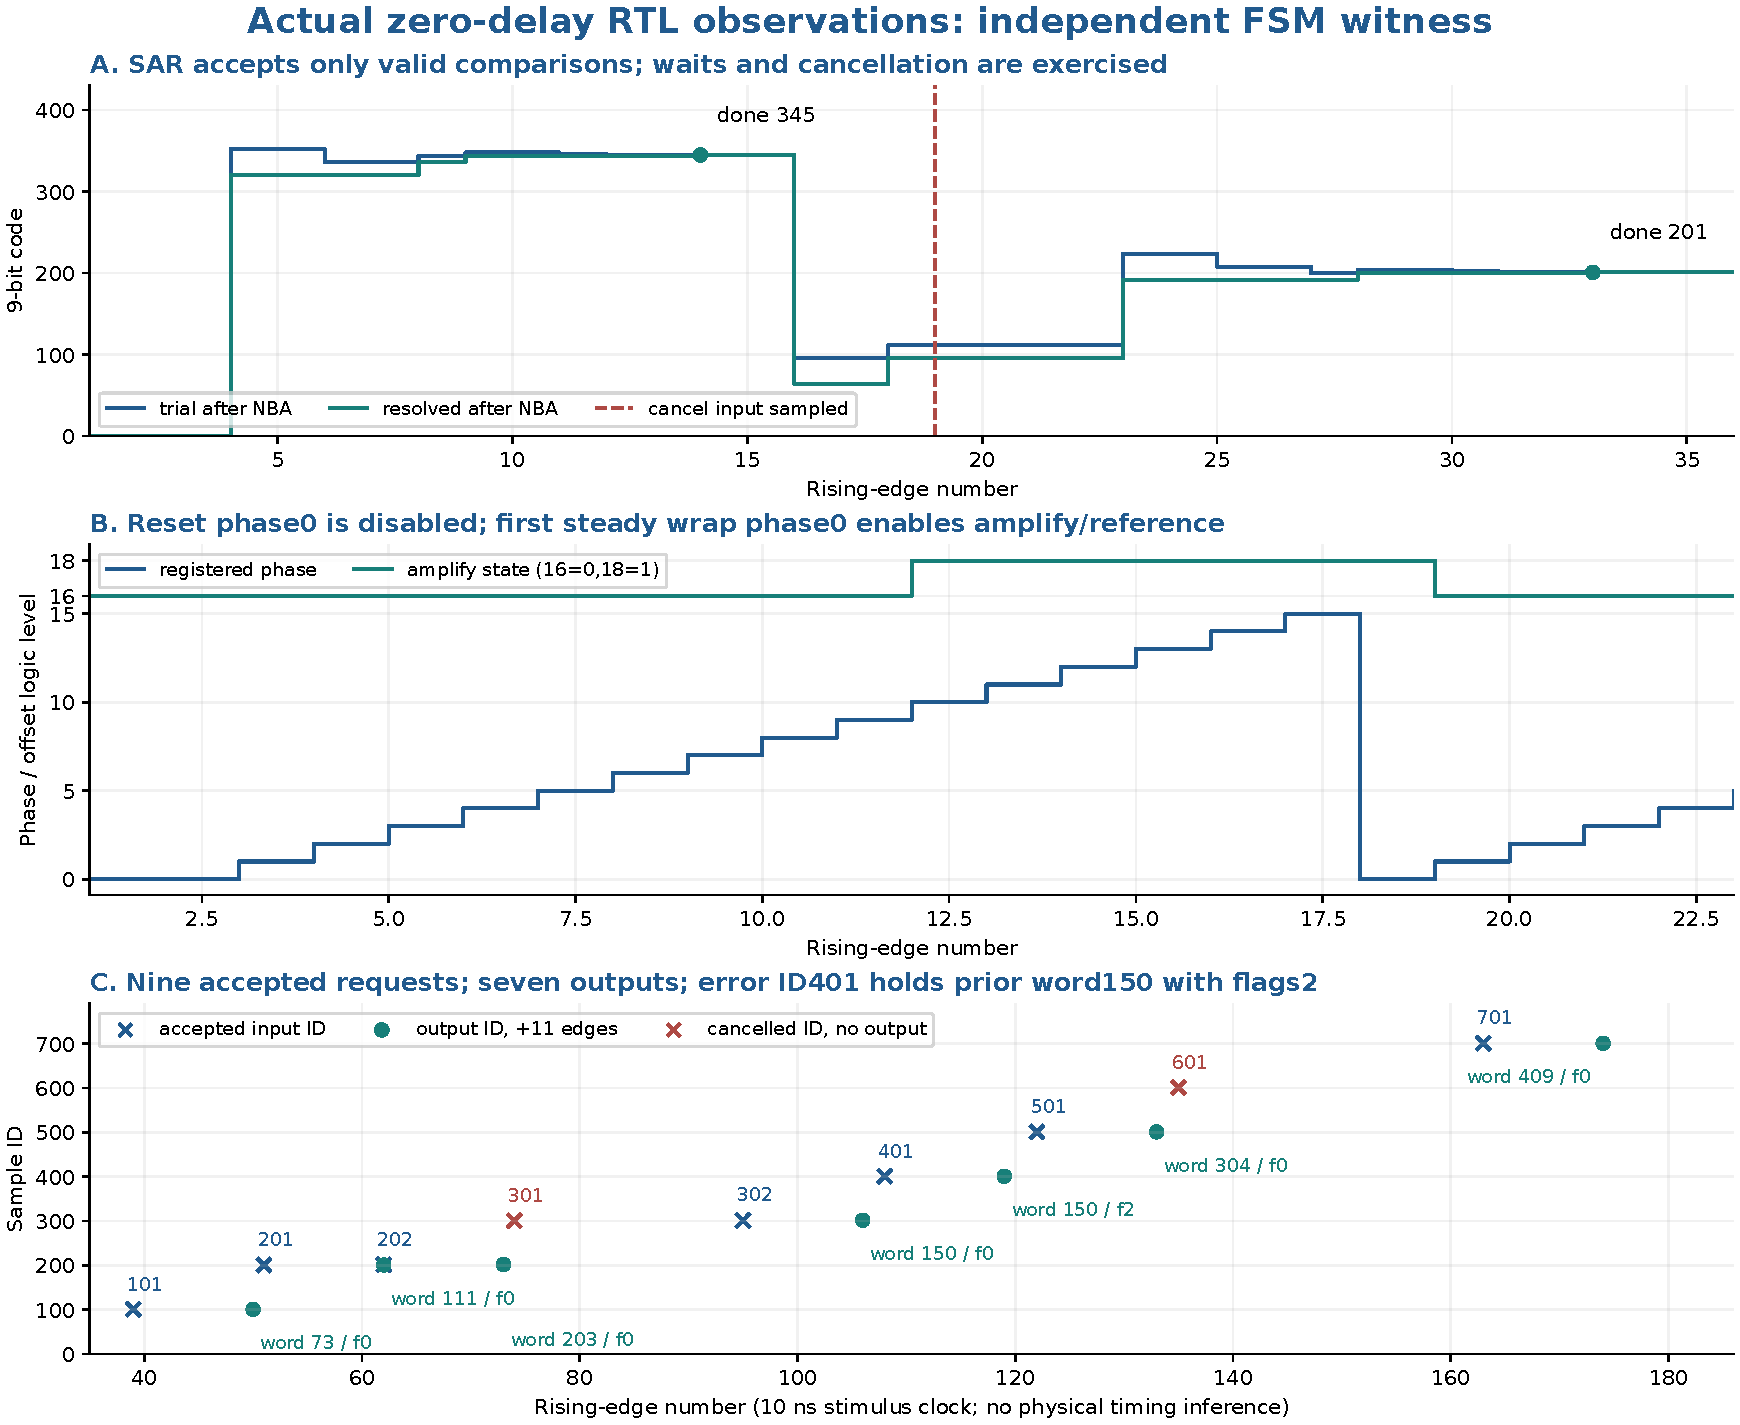
\includegraphics[width=0.96\textwidth]{figures/48_engineering_fsm_trace.pdf}
\caption{SAR接受、相位启动与重构完成事件的实际trace视图。它与前四幅解释图的角色不同：运行、来源SHA、信号记录时点及检查范围须同时绑定，不能由状态图插值或补画未观测值。}
\label{fig:eng-trace}
\end{figure}

实际数据来自\code{docs/evidence/20261001/engineering_fsm/}，官方Verilator 5.020与\code{engineering_fsm_tb}，三份CSV各175个上升沿。输入只在下降沿改变，记录上升沿前输入、接受条件和内部状态，再于NBA完成后1\,ps记录输出；10\,ns仅为仿真激励时钟，不能从零延迟仿真推导物理Fmax。重构使用1活跃slice、2主单位和1子单位的小几何，权重总和为$2^{30}$，使合法情况下输出与独立期望整数一致。它不替代18$\times$71的完整顶层回归或综合网表见证。

独立scoreboard按接受沿加11拍预约结果，不用DUT的div\_done决定期望完成时间。本轮9次接受、7次输出、2次取消（ID301/601）、1次错误输出（ID401）、1次同沿提交并接受下一笔。所有7笔有效输出延迟11拍；ID401的非法物理地址实际保持此前合法word150且flags=2，避免仅用旧零字形成弱断言。第62沿提交ID201、word111，同时捕获ID202、输入word203；后者在第73沿才提交。运行中取消及原定错误提交沿取消均无迟到输出，随后恢复成功。

SAR实际完成目标345与201，另有9个等待沿、1次取消和2次忙时start忽略；phase区分首次启动、10次稳态wrap和disable归零。图\ref{fig:eng-recon-boundary}保留沿前输入与沿后状态，能检查最后除法计算、输出提交和新接受之间的关系。CSV之外的未观测电气值没有插值加入。来源文件逐项SHA在\code{source_sha256.json}，原运行命令、构建/执行日志、摘要及哈希索引一并保存；制图脚本另逐项复算ID、码、flags、取消、延迟和完整边沿序列。

\begin{figure}[H]\centering
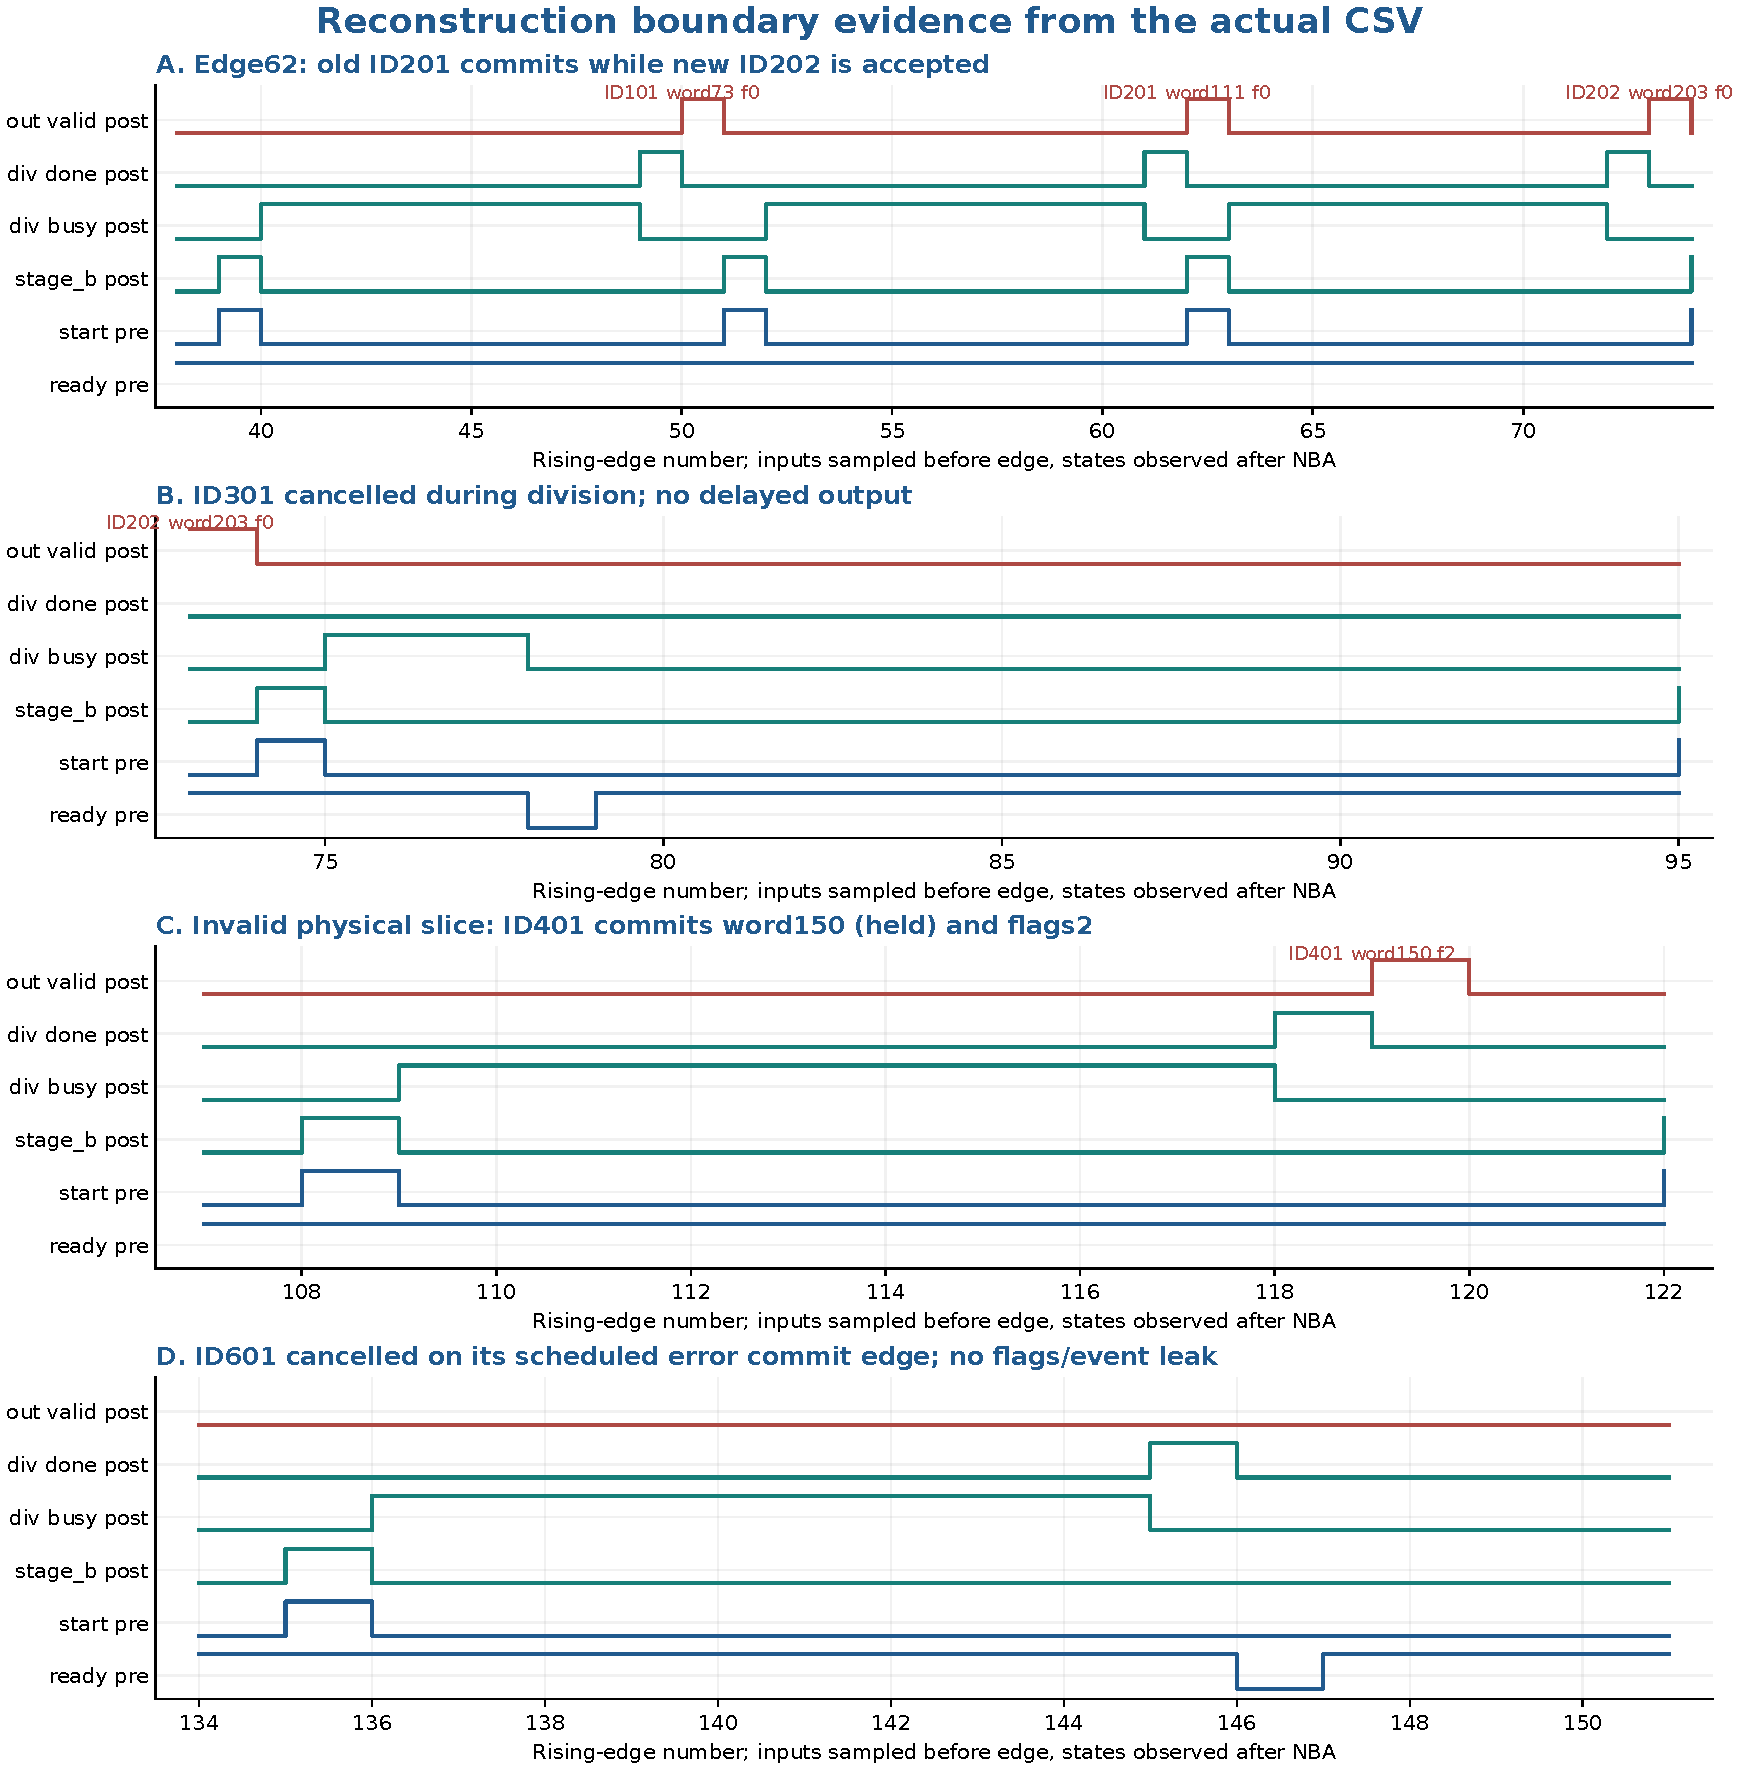
\includegraphics[width=0.96\textwidth]{figures/49_reconstruction_boundary_trace.pdf}
\caption{来自实际重构CSV的四段边界记录：旧结果提交与新start同沿、运行中取消、非法slice错误提交、错误提交沿取消。输入为沿前值，状态为NBA后值；不含SDF或模拟宏。}
\label{fig:eng-recon-boundary}
\end{figure}

\section{源码恒等复核如何连接原有物理证据}
\code{tools/audit_rtl_readability.py}逐文件读取\code{71e7d5a}的Git对象，检查全部26文件的有效token、字符串、语义pragma和预处理行；另用官方Verilator展开两套完整源列表，比较展开后的有效token。结果18,149个token恒等，25文件仅注释/空白变更，自动生成参数头字节不变。10个测试实例（1个排版正例、8个扰动负例与1组异常拒绝）覆盖运算符、常量、字符串、工具pragma、宏行边界、escaped identifier及不支持字符/续行的可见拒绝。本方法针对仓库有限SV子集，并非任意SV解析器或Formality签核。

当前RTL文件内容摘要见本次交付清单及\code{docs/evidence/20261001/rtl_readability/reviewed_result.json}。历史共享读选综合、网表及布线仍保留原\code{89b9f8153fea}\ldots{}源码身份，不能把新注释版的raw SHA写进旧实验。三类严格lint与新增bench已按本轮源文件重新编译；完整23项回归的GitHub结果另绑定本次提交。源码词法恒等建立阅读版与原硬件的关系，但没有宣称再次运行Vivado或产生新的时序/面积收益。若后续修改有效token、参数、宏、文件列表或语义指令，必须重建功能和物理证据链。
